\documentclass[12pt,a4paper]{article}
\usepackage[utf8]{vietnam}
\usepackage{amsmath,amssymb}
\usepackage{tabularx}
\usepackage{tikz}
\usetikzlibrary{calc,angles,quotes,arrows.meta}
\usepackage{xcolor}
\usepackage{enumitem}
\usepackage{fancyhdr}
\usepackage[top=1.2cm, bottom=1.2cm, left=1.5cm, right=1.5cm]{geometry}
\usepackage[dethi]{ex_test}
\SAOPTN{widthSA=2.6,heightSA=0.62}

\setlength{\headheight}{15pt}
\setlength{\parskip}{0pt}

% Dòng kẻ chấm mờ chuẩn viết tay
\newcommand{\dongke}[1]{%
  \begingroup%
  \setlength{\parskip}{0pt}%
  \baselineskip=18.5pt%
  \vspace{1.0mm}%
  \foreach \i in {1,...,#1}{%
    \noindent{\color{gray!60}\dotfill}\par%
  }%
  \vspace{0.6mm}%
  \endgroup%
}

\pagestyle{fancy}
\fancyhf{}
\rhead{\textit{Môn Toán 7 -- Đề số 4}}
\lhead{\textit{Bộ đề ôn tập Giữa học kì I}}
\cfoot{\thepage}

\begin{document}

% --- KHUNG TIÊU ĐỀ ĐỀ THI ---
\noindent
\begin{tabularx}{\linewidth}{X r}
\textbf{TRƯỜNG THCS: \dotfill} & \textbf{ĐỀ KIỂM TRA ĐỊNH KỲ GIỮA HỌC KỲ I} \\
\textbf{Họ và tên: \dotfill} & \textbf{NĂM HỌC 2026 -- 2027} \\
\textbf{Lớp: \dotfill \quad SBD: \dotfill} & \textbf{Môn: TOÁN 7} \\
& \textit{Thời gian làm bài: 90 phút (không kể thời gian phát đề)}
\end{tabularx}

\vspace{1.5mm}
\noindent
\begin{tabularx}{\linewidth}{|p{3.5cm}|X|}
\hline
\centering\textbf{Điểm số} & \centering\textbf{Lời nhận xét của thầy cô giáo} \tabularnewline
\rule{0pt}{1.6cm} & \\
\hline
\end{tabularx}

\vspace{2.5mm}
\begin{center}
\textbf{\large ĐỀ SỐ 4}
\end{center}

\noindent\textbf{\large PHẦN I. CÂU TRẮC NGHIỆM NHIỀU PHƯƠNG ÁN LỰA CHỌN (3,0 điểm)}

\textit{Thí sinh trả lời từ câu 1 đến câu 12. Mỗi câu hỏi chỉ chọn một phương án đúng nhất và ghi vào bảng đáp án.}

\vspace{1mm}
\begin{ex}
Chọn câu trả lời đúng: Trong định lí: ``Nếu một đường thẳng vuông góc với một trong hai đường thẳng song song thì nó cũng vuông góc với đường thẳng kia''. Ta có giả thiết là:
\choice
{``Nếu một đường thẳng vuông góc''}
{``Nó cũng vuông góc với đường thẳng kia''}
{``Nếu một đường thẳng vuông góc với một trong hai đường thẳng song song thì nó cũng vuông góc với đường thẳng kia''}
{\True ``Một đường thẳng vuông góc với một trong hai đường thẳng song song''}
\end{ex}

\begin{ex}
Số nào là số vô tỉ?
\choice
{$3{,}2$}
{$5{,}3(2)$}
{$0{,}6$}
{\True $-1{,}23427232\dots$}
\end{ex}

\begin{ex}
Số đối của số hữu tỉ $-0{,}25$ là:
\choice
{$-0{,}25$}
{$-\dfrac{1}{4}$}
{$-4$}
{\True $0{,}25$}
\end{ex}

\begin{ex}
Qua một điểm ở ngoài đường thẳng, ta kẻ được bao nhiêu đường thẳng song song với đường thẳng đó?
\choice
{$0$}
{\True $1$}
{$2$}
{$3$}
\end{ex}

\begin{ex}
Kết quả của phép tính $2^2 \cdot 2^5$ là:
\choice
{$2^{10}$}
{$2^3$}
{$2^5$}
{\True $2^7$}
\end{ex}

\begin{ex}
Cho hai số hữu tỉ $a$ và $b$ được biểu diễn trên trục số như sau. Chọn khẳng định đúng:
\begin{center}
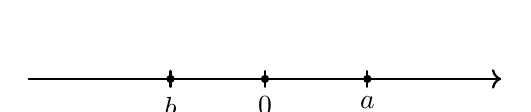
\begin{tikzpicture}[scale=1, line cap=round, line join=round]
  \draw[->, thick] (-3,0) -- (3,0);
  \draw[thick] (-1.2, -0.1) -- (-1.2, 0.1);
  \fill (-1.2, 0) circle (1.5pt);
  \node[below=3pt] at (-1.2, 0) {$b$};

  \draw[thick] (0, -0.1) -- (0, 0.1);
  \fill (0, 0) circle (1.5pt);
  \node[below=3pt] at (0, 0) {$0$};

  \draw[thick] (1.3, -0.1) -- (1.3, 0.1);
  \fill (1.3, 0) circle (1.5pt);
  \node[below=3pt] at (1.3, 0) {$a$};
\end{tikzpicture}
\end{center}
\choice
{$b > a > 0$}
{$b > a$}
{$b < a < 0$}
{\True $b < 0 < a$}
\end{ex}

\begin{ex}
\immini{
Tia phân giác của $\widehat{xOm}$ và $\widehat{yOn}$ lần lượt là:
\choice
{\True $Ok$ và $Ou$}
{$Ox$ và $Oy$}
{$Ou$ và $Om$}
{$Ok$ và $On$}
}{
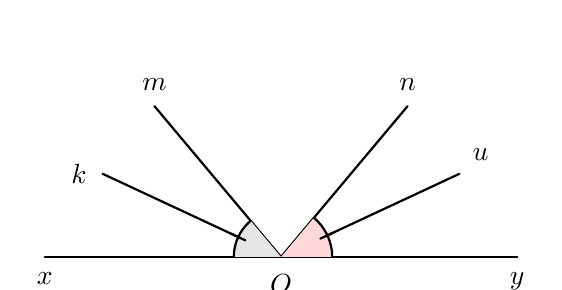
\begin{tikzpicture}[scale=1, line cap=round, line join=round]
  \coordinate (O) at (0,0);
  \draw[thick] (-3,0) node[below=2pt] {$x$} -- (3,0) node[below=2pt] {$y$};
  \draw[thick] (O) -- (130:2.5) node[above=2pt] {$m$};
  \draw[thick] (O) -- (155:2.5) node[left=2pt] {$k$};
  \draw[thick] (O) -- (50:2.5) node[above=2pt] {$n$};
  \draw[thick] (O) -- (25:2.5) node[above right=1pt] {$u$};

  \fill[gray!20] (O) -- (180:0.6) arc (180:130:0.6) -- cycle;
  \draw[thick] (180:0.6) arc (180:130:0.6);
  \draw[thick] (155:0.5) -- (155:0.7);

  \fill[red!15] (O) -- (0:0.65) arc (0:50:0.65) -- cycle;
  \draw[thick] (0:0.65) arc (0:50:0.65);
  \draw[thick] (25:0.55) -- (25:0.75);

  \node[below=3pt] at (O) {$O$};
\end{tikzpicture}
}
\end{ex}

\begin{ex}
Cho một hình lăng trụ đứng có diện tích đáy là $S$, chiều cao là $h$. Công thức tính thể tích của hình lăng trụ đứng là:
\choice
{\True $V = S \cdot h$}
{$V = \dfrac{1}{2} S \cdot h$}
{$V = 2 S \cdot h$}
{$V = 3 S \cdot h$}
\end{ex}

\begin{ex}
Tính $\left[ \left(\dfrac{1}{3}\right)^2 \right]^4$ ta được:
\choice
{$\left(\dfrac{1}{3}\right)^2$}
{\True $\left(\dfrac{1}{3}\right)^8$}
{$\left(\dfrac{1}{3}\right)^6$}
{$\left(\dfrac{1}{3}\right)^4$}
\end{ex}

\begin{ex}
Có bao nhiêu giá trị của $x \in \mathbb{Q}; x \ge 1$ sao cho $x^4 - x = 0$?
\choice
{\True $1$}
{$0$}
{$2$}
{$3$}
\end{ex}

\begin{ex}
\immini{
Cho hình vẽ sau, biết $Ob$ là tia phân giác của $\widehat{aOc}$. Khẳng định nào sau đây đúng?
\choice
{$\widehat{bOc} = 90^\circ$}
{\True $\widehat{bOc} = 60^\circ$}
{$\widehat{bOc} = 30^\circ$}
{$\widehat{bOc} = 120^\circ$}
}{
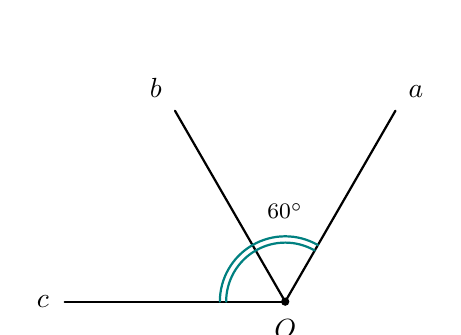
\begin{tikzpicture}[scale=1, line cap=round, line join=round]
  \coordinate (O) at (0,0);
  \draw[thick] (O) -- (-2.8,0) node[left=2pt] {$c$};
  \draw[thick] (O) -- (120:2.8) node[above left=1pt] {$b$};
  \draw[thick] (O) -- (60:2.8) node[above right=1pt] {$a$};

  \fill (O) circle (1.5pt) node[below=3pt] {$O$};

  \draw[teal, thick] (60:0.75) arc (60:120:0.75);
  \draw[teal, thick] (60:0.83) arc (60:120:0.83);
  \node[font=\footnotesize] at (90:1.15) {$60^\circ$};

  \draw[teal, thick] (120:0.75) arc (120:180:0.75);
  \draw[teal, thick] (120:0.83) arc (120:180:0.83);
\end{tikzpicture}
}
\end{ex}

\begin{ex}
Trong các số sau, số nào là số vô tỉ?
\choice
{$-5$}
{$5{,}7$}
{\True $\sqrt{7}$}
{$\dfrac{5}{3}$}
\end{ex}


\vspace{1mm}
\noindent\textbf{BẢNG TRẢ LỜI TRẮC NGHIỆM PHẦN I:}
\begin{center}
\begin{tabular}{|c|c|c|c|c|c|c|c|c|c|c|c|c|}
\hline
\textbf{Câu} & \textbf{1} & \textbf{2} & \textbf{3} & \textbf{4} & \textbf{5} & \textbf{6} & \textbf{7} & \textbf{8} & \textbf{9} & \textbf{10} & \textbf{11} & \textbf{12} \\
\hline
\textbf{Chọn} & \rule{0pt}{0.65cm} & & & & & & & & & & & \\
\hline
\end{tabular}
\end{center}
\vspace{2mm}

\setcounter{ex}{0}
\noindent\textbf{\large PHẦN II. CÂU TRẮC NGHIỆM ĐÚNG SAI (2,0 điểm)}

\textit{Thí sinh trả lời câu 1 và câu 2. Trong mỗi ý a), b), c), d) ở mỗi câu, thí sinh chọn đúng hoặc sai.}

\vspace{1mm}
\begin{ex}
Cho $a, b, c, d \in \mathbb{Q}$. Xét tính đúng sai của các mệnh đề sau:
\choiceTF
{\True Bỏ dấu ngoặc của biểu thức $-(a + b - c)$ ta được kết quả $-a - b + c$}
{Bỏ dấu ngoặc của biểu thức $a + (-b - c + d)$ ta được kết quả $a - b - c - d$}
{Cho $a + b = c$, áp dụng quy tắc chuyển vế ta được $a = -b - c$}
{\True Cho $a - \dfrac{3}{4} = 5$, áp dụng quy tắc chuyển vế ta được $a = 5 + \dfrac{3}{4}$}
\end{ex}

\begin{ex}
\immini{
Quan sát hình vẽ, hai đường thẳng $a$ và $b$ cắt nhau tại điểm $O$ tạo thành bốn góc $\widehat{O}_1, \widehat{O}_2, \widehat{O}_3, \widehat{O}_4$. Xét tính đúng sai của các mệnh đề sau:
\choiceTF
{\True Góc $\widehat{O}_1$ và góc $\widehat{O}_3$ là hai góc đối đỉnh}
{Góc $\widehat{O}_2$ và góc $\widehat{O}_4$ là hai góc kề bù}
{\True Tổng số đo của góc $\widehat{O}_1$ và góc $\widehat{O}_2$ bằng $180^\circ$}
{\True Nếu số đo góc $\widehat{O}_1$ bằng $60^\circ$ thì số đo góc $\widehat{O}_4$ bằng $120^\circ$}
}{
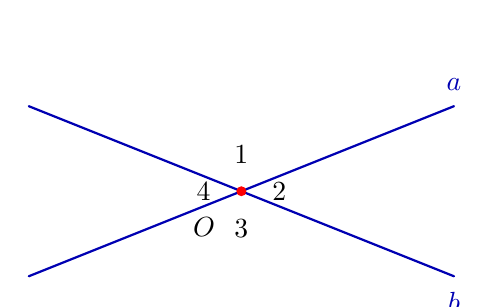
\begin{tikzpicture}[scale=0.9, line cap=round, line join=round]
  \coordinate (O) at (0,0);
  \draw[thick, blue!70!black] (-3,-1.2) -- (3,1.2) node[above=2pt] {$a$};
  \draw[thick, blue!70!black] (-3,1.2) -- (3,-1.2) node[below=2pt] {$b$};

  \fill[red] (O) circle (2pt);

  \node[above=2pt] at (0,0.18) {$1$};
  \node[right=2pt] at (0.22,0) {$2$};
  \node[below=2pt] at (0,-0.18) {$3$};
  \node[left=2pt] at (-0.22,0) {$4$};

  \node[below left=6pt] at (O) {$O$};
\end{tikzpicture}
}
\end{ex}


\noindent\textbf{BẢNG TRẢ LỜI PHẦN II:}
\begin{center}
\begin{tabular}{|c|c|c|c|c||c|c|c|c|c|}
\hline
\textbf{Câu 1} & \textbf{a)} & \textbf{b)} & \textbf{c)} & \textbf{d)} & \textbf{Câu 2} & \textbf{a)} & \textbf{b)} & \textbf{c)} & \textbf{d)} \\
\hline
\textbf{Đ/S} & \rule{0pt}{0.6cm} & & & & \textbf{Đ/S} & & & & \\
\hline
\end{tabular}
\end{center}
\vspace{2mm}

\setcounter{ex}{0}
\noindent\textbf{\large PHẦN III. CÂU HỎI TRẢ LỜI NGẮN (1,0 điểm)}

\textit{Thí sinh trả lời câu 1 và câu 2. Điền kết quả vào ô trống.}

\vspace{1mm}
\begin{ex}
Tính hợp lý giá trị của biểu thức: $A = \dfrac{-5}{9} \cdot \dfrac{4}{13} + \dfrac{-5}{9} \cdot \dfrac{9}{13} + \dfrac{5}{9}$. \shortans{$0$}
\end{ex}

\begin{ex}
Cho hai góc kề bù $\widehat{AOB}$ và $\widehat{BOC}$, biết $\widehat{AOB} = 110^\circ$. Gọi $OM$ là tia phân giác của $\widehat{AOB}$. Tính số đo góc $\widehat{BOC}$ và $\widehat{COM}$. \shortans{$\widehat{BOC} = 70^\circ; \widehat{COM} = 125^\circ$}
\end{ex}


\setcounter{ex}{0}
\noindent\textbf{\large PHẦN IV. TỰ LUẬN (4,0 điểm)}

\textit{Thí sinh trình bày chi tiết lời giải vào giấy làm bài.}

\vspace{1mm}
\begin{ex}
Thực hiện phép tính:
\begin{enumerate}[label=\textbf{\alph*)}, leftmargin=0.8cm, itemsep=1pt]
\item $\dfrac{5}{12} + \left(-\dfrac{7}{24}\right) : \dfrac{3}{8}$
\item $\left(-\dfrac{4}{5}\right) \cdot \dfrac{3}{7} - \dfrac{4}{7} : \sqrt{\dfrac{25}{16}} - |-1|$
\end{enumerate}
\end{ex}
\vspace{1.5mm}

\begin{ex}
Tìm $x$ biết:
\begin{enumerate}[label=\textbf{\alph*)}, leftmargin=0.8cm, itemsep=1pt]
\item $\dfrac{3}{5} x + \dfrac{2}{3} = \dfrac{2^3}{3}$
\item $2 \sqrt{x} - 1 = 0$
\end{enumerate}
\end{ex}
\vspace{1.5mm}

\begin{ex}
Một siêu thị nhập vào 250 hộp bánh với giá bán niêm yết là 120 000 đồng/hộp. Đợt thứ nhất siêu thị bán được $\dfrac{3}{5}$ số hộp bánh với đúng giá niêm yết. Đợt thứ hai vì muốn kích cầu tiêu dùng, siêu thị đã giảm giá 8\% so với giá niêm yết ban đầu và đã bán hết số hộp bánh còn lại.
\begin{enumerate}[label=\textbf{\alph*)}, leftmargin=0.8cm, itemsep=1pt]
\item Hỏi đợt thứ nhất siêu thị đã bán được bao nhiêu hộp bánh và thu về được bao nhiêu tiền?
\item Cả hai đợt siêu thị đã thu về được bao nhiêu tiền?
\end{enumerate}
\end{ex}
\vspace{1.5mm}

\begin{ex}
\immini{
Cho tam giác $ABC$ có $BA = BC$. Gọi $M$ là trung điểm của đoạn thẳng $AC$. Chứng minh rằng: $\widehat{ABM} = \widehat{CBM}$.
}{
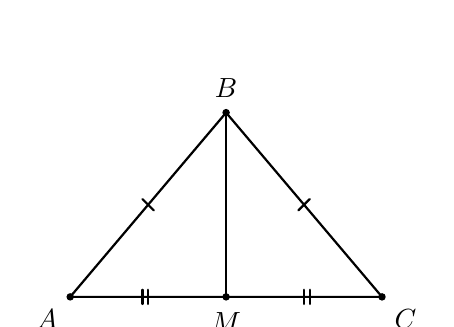
\begin{tikzpicture}[scale=0.9, line cap=round, line join=round]
  \coordinate (B) at (0,2.6);
  \coordinate (A) at (-2.2,0);
  \coordinate (C) at (2.2,0);
  \coordinate (M) at (0,0);

  \draw[thick] (A) -- (B) -- (C) -- cycle;
  \draw[thick] (B) -- (M);

  \fill (A) circle (1.5pt) node[below left=1pt] {$A$};
  \fill (B) circle (1.5pt) node[above=2pt] {$B$};
  \fill (C) circle (1.5pt) node[below right=1pt] {$C$};
  \fill (M) circle (1.5pt) node[below=2pt] {$M$};

  \draw[thick] ($(A)!0.5!(B)+(-0.08,0.08)$) -- ($(A)!0.5!(B)+(0.08,-0.08)$);
  \draw[thick] ($(C)!0.5!(B)+(-0.08,-0.08)$) -- ($(C)!0.5!(B)+(0.08,0.08)$);

  \draw[thick] (-1.1,-0.1) -- (-1.1,0.1);
  \draw[thick] (-1.18,-0.1) -- (-1.18,0.1);
  \draw[thick] (1.1,-0.1) -- (1.1,0.1);
  \draw[thick] (1.18,-0.1) -- (1.18,0.1);
\end{tikzpicture}
}
\end{ex}
\vspace{1.5mm}


\begin{center}
\rule{4cm}{0.4pt}\\
\textit{--- HẾT ---}
\end{center}
\end{document}
